\chapter{Multiple selection problem}
\label{tree:MS}

The multiple selection problem is depicted as follows,

Find the $k$ elements at positions $p_1, \dots, p_k \in P$ in a permutation of array $A$ that respects the following constraints,

\begin{equation}
\forall_{p_k \in P}\forall_{i = 0}^{i < p_k} \text{comp}(A_i, A_{p_k})
\end{equation}

\begin{equation}
\forall_{p_k \in P}\forall_{i = p_k + 1}^{i < |A| - 1} \neg\text{comp}(A_i, A_{p_k})
\end{equation}

where the comparison operator is usually $\leq$.\\


\begin{figure}
	\centering
	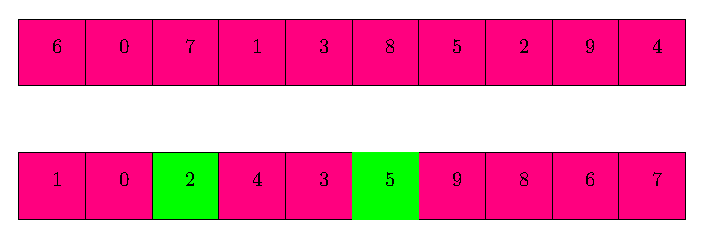
\includegraphics[width=0.5\textwidth]{fig/ms:array}
	\caption{\label{fig:ms:array} An array of 10 elements and its multiple selection result.}
\end{figure}


\begin{theorem}
The ITLB for the multiple selection problem lies between $n$ and $n \log n$ and depends on $P$.
\end{theorem}

\begin{proof}\mbox{}\\*
\begin{enumerate}
\item Notice that the sorting problem is a special case of the multiple selection problem where $P = \{0,\dots,|A|\}$.
\item Notice that the selection problem is a special case of the multiple selection problem where $|P| = 1$.
\end{enumerate}
\end{proof}

The Hasse diagrams for this problem are those in \ref{fig:ms:diag}.

\begin{figure}
	\centering
	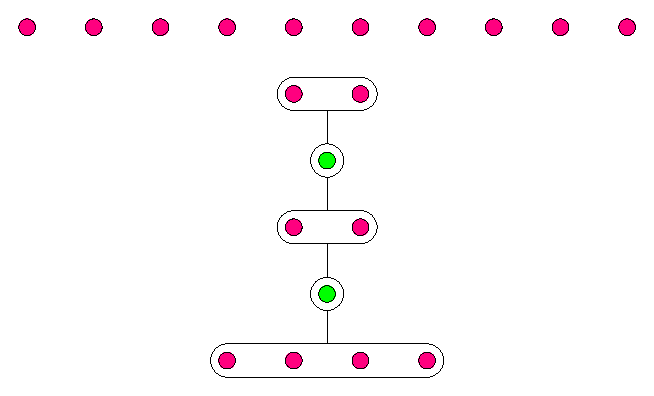
\includegraphics[width=0.6\textwidth]{fig/ms:diag}
	\caption{\label{fig:ms:diag} Hasse diagrams for the multiple selection problem.}
\end{figure}